% sections/06_data_structures.tex

\section{Proposed Data Structures}

% --- Slide: HT Architecture ---
\begin{frame}[t]{The Hash Tree (HT): Internal Architecture}
    \begin{columns}
        \begin{column}{0.5\textwidth}
            \begin{itemize}
                \item \textbf{Routing Logic:} Internal nodes use a hash function $h(i)$ to select the branch.
                \item \textbf{Leaf Buckets:} Fixed-size containers for candidate verification.
            \end{itemize}
        \end{column}
        \begin{column}{0.5\textwidth}
            \centering
            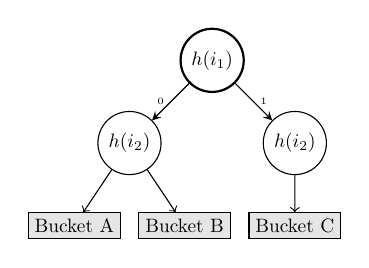
\begin{tikzpicture}[scale=0.7, every node/.style={scale=0.7}]
                \node[draw, circle, thick] (R) at (2,3) {$h(i_1)$};
                \node[draw, circle] (C1) at (0.5,1.5) {$h(i_2)$};
                \node[draw, circle] (C2) at (3.5,1.5) {$h(i_2)$};
                \node[draw, rectangle, fill=gray!20] (L1) at (-0.5,0) {Bucket A};
                \node[draw, rectangle, fill=gray!20] (L2) at (1.5,0) {Bucket B};
                \node[draw, rectangle, fill=gray!20] (L3) at (3.5,0) {Bucket C};
                
                \draw[->, >=stealth] (R) -- (C1) node[midway, left] {\tiny 0};
                \draw[->, >=stealth] (R) -- (C2) node[midway, right] {\tiny 1};
                \draw[->] (C1) -- (L1);
                \draw[->] (C1) -- (L2);
                \draw[->] (C2) -- (L3);
            \end{tikzpicture}
        \end{column}
    \end{columns}
    \vfill
    \begin{alertblock}{Design Intent}
        To verify $\{1, 5\}$, the system calculates $h(1)$ then $h(5)$ to reach a specific bucket. This minimizes memory footprint but increases computational cost.
    \end{alertblock}
\end{frame}

% --- Slide: HT Bottlenecks ---
\begin{frame}[t]{The Hash Tree (HT): Performance Bottlenecks}
    \begin{alertblock}{The "Bucket Overflow" Phenomenon}
        When $h(i)$ produces collisions, the leaf bucket becomes a long linked list.
    \end{alertblock}

    \begin{itemize}
        \item \textbf{Search Breakdown:} Verification degrades from a "smart jump" to a \textbf{linear scan} ($O(n)$).
        \item \textbf{The Spark Tax:} On Spark RDDs, the constant calculation of $h(i)$ for millions of records creates a bottleneck that prevents high-throughput scaling.
    \end{itemize}
    
    \vfill
    \centering
    \begin{tikzpicture}[scale=0.9]
        \node[draw, rectangle, minimum width=3.5cm, fill=red!10, thick] (B) {Bucket Overflow};
        \node[draw, rectangle, right=0.5cm of B, font=\tiny] (i1) {$\{a,b,c\}$};
        \node[draw, rectangle, right=0cm of i1, font=\tiny] (i2) {$\{a,d,e\}$};
        \node[draw, rectangle, right=0cm of i2, font=\tiny] (i3) {$\{b,c,e\}$};
        \node[draw, rectangle, right=0cm of i3, font=\tiny] (i4) {\dots};
        \draw[thick, red, ->] (B.east) -- (i1.west);
    \end{tikzpicture}
\end{frame}

% --- Slide: The Trie ---
\begin{frame}[t]{The Trie (Prefix Tree): Structural Optimization}
    \begin{columns}
        \begin{column}{0.4\textwidth}
            \textbf{Prefix Sharing:}
            \begin{itemize}
                \item Itemsets: $\{a,b,c\}$ and $\{a,b,d\}$.
                \item $\{a,b\}$ is stored once, exploiting commonality.
            \end{itemize}
        \end{column}
        \begin{column}{0.6\textwidth}
            \centering
            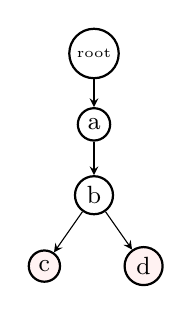
\begin{tikzpicture}[
                node/.style={draw, circle, inner sep=2pt, font=\small, thick},
                edge/.style={->, >=stealth},
                scale=0.9
            ]
                \node[node] (R) at (0,0) {\tiny root};
                \node[node] (A) at (0,-1) {a};
                \node[node] (B) at (0,-2) {b};
                \node[node, fill=red!5] (C) at (-0.7,-3) {c};
                \node[node, fill=red!5] (D) at (0.7,-3) {d};
                
                \draw[edge] (R) -- (A);
                \draw[edge] (A) -- (B);
                \draw[edge] (B) -- (C);
                \draw[edge] (B) -- (D);
            \end{tikzpicture}
        \end{column}
    \end{columns}
    \vfill
    \begin{alertblock}{The Sibling Problem}
        Finding 'd' after 'b' requires searching through all of 'b's children. In large datasets, this search is $O(\log k)$ or $O(k)$ depending on the node implementation.
    \end{alertblock}
\end{frame}

% --- Slide: The HTT Solution ---
\begin{frame}[t]{The Hash Table Trie (HTT) Hybrid}
    \vspace{-0.2cm}
    \textbf{The Innovation: Localized Map Lookup}
    
    \begin{center}
    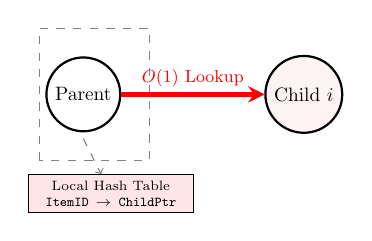
\begin{tikzpicture}[scale=0.7, every node/.style={transform shape}]
        \node[draw, circle, thick] (P) at (0,0) {Parent};
        \node[draw, circle, thick, fill=red!5] (C) at (4,0) {Child $i$};
        
        \draw[dashed, gray] (-0.8,-1.2) rectangle (1.2,1.2);
        \node[draw, rectangle, fill=red!10, minimum width=3cm, align=center, font=\scriptsize] (HT) at (0.5,-1.8) {Local Hash Table\\ \texttt{ItemID $\rightarrow$ ChildPtr}};
        
        \draw[->, ultra thick, red, >=stealth] (P) -- (C) node[midway, above] {\small $O(1)$ Lookup};
        \draw[->, thin, gray, dashed] (0,-0.8) -- (HT);
    \end{tikzpicture}
    \end{center}

    \vspace{-0.4cm}

    \begin{table}[]
        \centering
        \scriptsize
        \begin{tabular}{l|c|c|c}
            \toprule
            \textbf{Metric} & \textbf{HT} & \textbf{Standard Trie} & \textbf{HTT (Proposed)} \\ \midrule
            Sibling Lookup & $O(n)$ scan & $O(\log k)$ search & $\mathbf{O(1)}$ \textbf{lookup} \\ 
            Traversal Time & $O(k \cdot h)$ & $O(L \cdot \log k)$ & $\mathbf{O(L)}$ \\ 
            Spark Reality & CPU Bound & Memory Latency & \textbf{Max Throughput} \\ \bottomrule
        \end{tabular}
    \end{table}

    \vspace{-0.2cm}

    \begin{alertblock}{Technical Verdict}
        By embedding hash tables \textit{inside} the Trie nodes, the \textbf{HTT} eliminates the branching factor ($k$) from the complexity, maximizing Spark's RDD throughput.
    \end{alertblock}
\end{frame}
